\documentclass[10pt]{beamer}
\usepackage{etex}
\usetheme[
%%% options passed to the outer theme
%    progressstyle=fixedCircCnt,   %either fixedCircCnt, movCircCnt, or corner
%    rotationcw,          % change the rotation direction from counter-clockwise to clockwise
%    shownavsym          % show the navigation symbols
  ]{AAUsimple}
  
% If you want to change the colors of the various elements in the theme, edit and uncomment the following lines
% Change the bar and sidebar colors:
%\setbeamercolor{AAUsimple}{fg=green!20,bg=green}
%\setbeamercolor{sidebar}{bg=red!20}
% Change the color of the structural elements:
%\setbeamercolor{structure}{fg=red}
% Change the frame title text color:
%\setbeamercolor{frametitle}{fg=blue}
% Change the normal text color background:
%\setbeamercolor{normal text}{fg=black,bg=gray!10}
% ... and you can of course change a lot more - see the beamer user manual.

\usepackage[utf8]{inputenc}
\usepackage[english]{babel}
\usepackage[T1]{fontenc}
% Or whatever. Note that the encoding and the font should match. If T1
% does not look nice, try deleting the line with the fontenc.
\usepackage{helvet}
\usepackage{xcolor}

%use for graphics
\usepackage{calc}
\usepackage{ifthen}
\usepackage{tikz}
%other package for graphics

%use for itemize style
%\usepackage{enumitem}

%\usepackage{pstricks}
%\usepackage{pstricks-add}

%\usepackage{pst-plot}
\usepackage{xcolor,colortbl}

\newcommand{\mc}[2]{\multicolumn{#1}{c}{#2}}
\definecolor{Gray}{gray}{0.85}

\newcolumntype{a}{>{\columncolor{Gray}}c}
\newcolumntype{b}{>{\columncolor{white}}c}

% command for slices graphic
\newcommand{\slice}[4]{
  \pgfmathparse{0.5*#1+0.5*#2}
  \let\midangle\pgfmathresult

  % slice
  \draw[thick,fill=black!10] (0,0) -- (#1:1) arc (#1:#2:1) -- cycle;

  % outer label
  \node[label=\midangle:#4] at (\midangle:1) {};

  % inner label
  \pgfmathparse{min((#2-#1-10)/110*(-0.3),0)}
  \let\temp\pgfmathresult
  \pgfmathparse{max(\temp,-0.5) + 0.8}
  \let\innerpos\pgfmathresult
  \node at (\midangle:\innerpos) {#3};
}
% colored hyperlinks
\newcommand{\chref}[2]{%
  \href{#1}{{\usebeamercolor[bg]{AAUsimple}#2}}%
}


\title{Implementing a Dynamic and Global\\ Scheduling Algorithm in a Real-Time OS}  % could also be a conference name
\subtitle{From theory to practice}
\date{August 25, 2017}
\author{
  Arabella Brayer
}
% - Give the names in the same order as they appear in the paper.
% - Use the \inst{?} command only if the authors have different
%   affiliation. See the beamer manual for an example

\institute[
%  {\includegraphics[scale=0.2]{aau_segl}}\\ %insert a company, department or university logo
  Computer Science Department
  Université Libre de Bruxelles
] % optional - is placed in the bottom of the sidebar on every slide
{% is placed on the bottom of the title page
  Computer Science Department \\
  Université Libre de Bruxelles \\

  
  %there must be an empty line above this line - otherwise some unwanted space is added between the university and the country (I do not know why;( )
}

% specify a logo on the titlepage (you can specify additional logos an include them in 
% institute command below
\pgfdeclareimage[height=1.5cm]{titlepagelogo}{img/ULB}% placed on the title page
\titlegraphic{% is placed on the bottom of the title page
  \pgfuseimage{titlepagelogo}
%  \hspace{1cm}\pgfuseimage{titlepagelogo2}
}
\definecolor{firstcolor}{RGB}{0, 76, 146}
\definecolor{secondcolor}{RGB}{126, 148, 0}
%\definecolor{secondcolor}{RGB}{43,46,62}
\definecolor{thirdcolor}{RGB}{180,200,212}
\newcommand{\emphS}[1]{\textcolor{olive}{#1}}
\begin{document}
% the titlepage
{\aauwavesbg%
\begin{frame}[plain,noframenumbering]
  \titlepage
\end{frame}}

\begin{frame}{Context}{Implementing a Dynamic and Global Scheduling Algorithm in RTOS}
  \begin{minipage}{0.6\textwidth}
    \begin{block}
    {RTOS}
      \begin{itemize}
          \item \emphS{R}eal-\emphS{T}ime \emphS{O}perating \emphS{S}ystem
            \begin{itemize}
              \setbeamertemplate{itemize items}[circle]
              \item \emphS{H}ard or \emphS{S}oft critical systems
            \end{itemize}
        \end{itemize}
      \end{block}
      \begin{block}
      {Scheduling}
      \begin{itemize}
          \item \emphS{M}ono-processor
          \item \emphS{M}ulti-processor
          \begin{itemize}
          \setbeamertemplate{itemize items}[circle]
            \item Partitioned
            \item Global
          \end{itemize}
      \end{itemize}
    \end{block}
  \end{minipage}
\end{frame}

\section{HIPPEROS}
\begin{frame}{HIPPEROS}{}
\begin{figure}[h]
	
\includegraphics[height=1cm]{img/HIPPEROS_logo_slogan}
\end{figure}
\begin{minipage}{0.6\textwidth}
\begin{block}{Internship}
    \begin{itemize}
      \item Knowledge of the \emphS{RTOS}
      \item ... specific aspects
    \end{itemize}
  \end{block}
\end{minipage}
\begin{minipage}{0.25\textwidth}
  \begin{block}{Internship}
  \end{block}
\end{minipage}
\end{frame}

\section{Work already done}
\begin{frame}{Work already done}{State of the art}
  \begin{minipage}{0.5\textwidth}
    \begin{block}
      {Choice of the algorithm} 
      \begin{itemize}
        \item There are plenty
        \item No ideal algorithm
        \item For interesting classes :
		\begin{itemize}
        \setbeamertemplate{itemize items}[circle]
        	\item Sporadic
            \item Arbitrary deadlines
        \end{itemize}
        \item Sober in migrations 
		\end{itemize}
    \end{block}
  \end{minipage}
  \begin{minipage}{0.4\textwidth}
  	\LARGE\emphS{QPS}
  \end{minipage}
\end{frame}

\begin{frame}{Work to do}{}
\begin{minipage}{0.5\textwidth}
 \begin{block}
 	{1 -- Implementation}
  \end{block}
  \begin{block}
  	{2 -- Benchmarks}
  \end{block}
  \begin{block}
  	{3 -- ... to be followed}
  \end{block}
\end{minipage}
\begin{minipage}{0.4\textwidth}
\begin{figure}[h]
	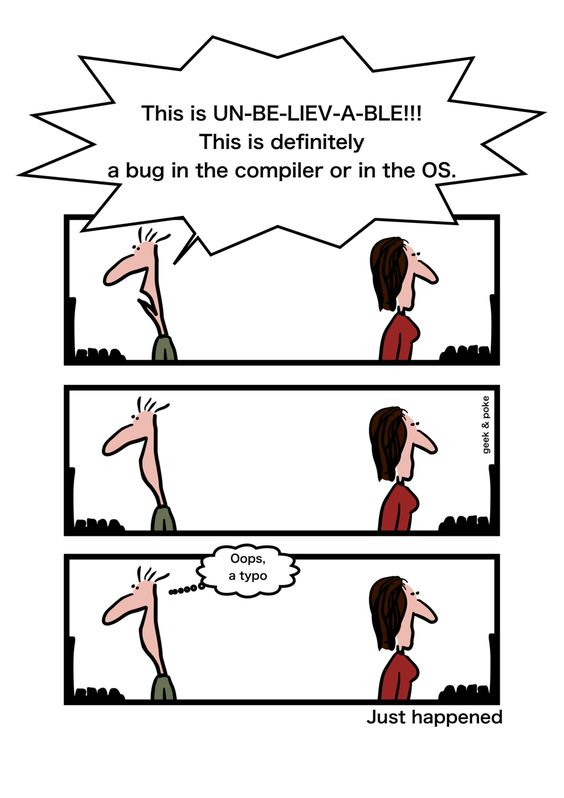
\includegraphics[height=6cm]{img/bug}
\end{figure}
\end{minipage}
\end{frame}

%%%%%%%%%%%%%%%% FIN PRES. %%%%%%%%%%%%%%%%%%%%%%%%%%

{\finalbg
\begin{frame}[plain,noframenumbering]
  \finalpage{Thank you!}
\end{frame}}
%%%%%%%%%%%%%%%%

\end{document}